\chapter{Music Notation Background}
\label{app:notation-primer}

Western staff notation is a two-dimensional visual code: it lays pitch along the
vertical axis of the page and time along the horizontal axis.
A note's \emph{height} on the staff fixes which pitch sounds; its \emph{horizontal}
placement and its drawn shape fix when the note starts and how long it lasts.
Reading a score is therefore the inverse of the problem this thesis automates:
recovering a symbolic pitch-and-time sequence from that two-dimensional image
(\Cref{ch:design}).
This appendix introduces, for readers without a musical background, the notation
elements that recovery must account for; familiarity with them informs the
vocabulary design, the data pipeline, and the error analysis of later chapters.
Readers already fluent in Western staff notation may skip this appendix without
loss.\todo{cite a standard notation reference (Gould, \emph{Behind Bars}; or Read, \emph{Music Notation}) somewhere in this appendix to ground the definitions.}

\section{The Staff, Clef, and Pitch}

Music is written on a \term{staff}: five horizontal lines and the four spaces between
them.
A note's vertical position on this grid encodes its pitch: moving a notehead up by one
line-or-space raises it by one diatonic step, i.e.\ to the next letter name.

The reference point is the \term{clef} at the left edge of the staff.
Lead sheets use the \term{treble clef} (or \term{G clef}) exclusively, the only clef
this thesis targets (\Cref{sec:scope}); its spiral encircles the second line from the
bottom and fixes it as G4, the G above middle C.
From that anchor the five lines spell, bottom to top, E4--G4--B4--D5--F5 (mnemonic
\emph{Every Good Boy Deserves Fudge}) and the four spaces spell F4--A4--C5--E5
(\emph{FACE}).
Pitches outside this range are written on short \term{ledger lines}: middle C (C4) sits
one ledger line below the staff, A5 one ledger line above it.
\Cref{fig:staff-pitches} traces the ascending C major scale from C4 to C5 across the
grid, making the pitch--position correspondence explicit.

\begin{figure}[htbp]
    \centering
    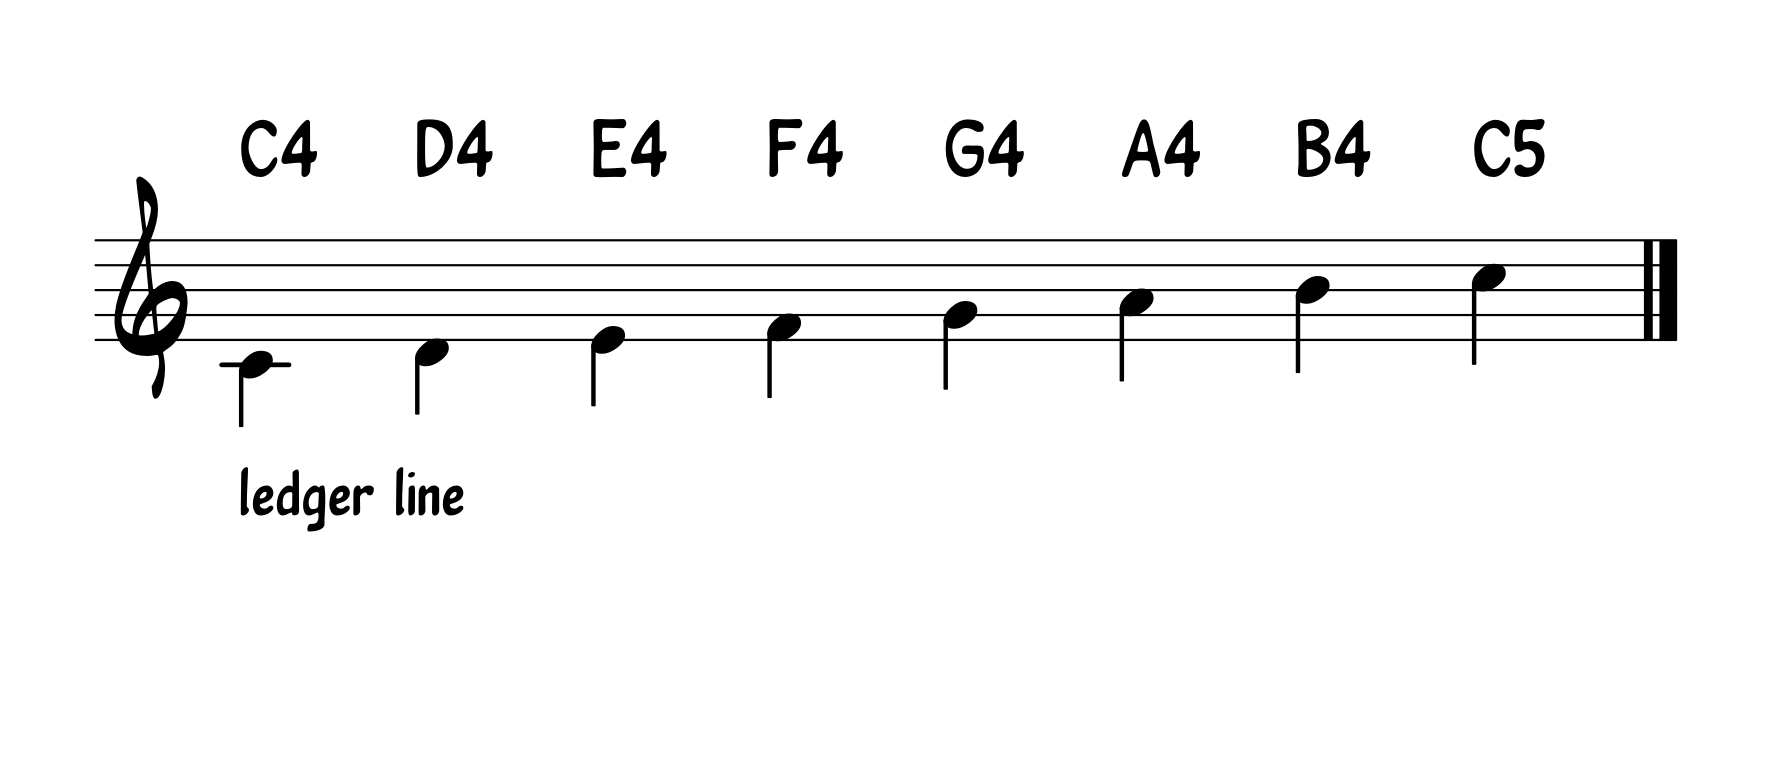
\includegraphics[width=0.82\textwidth]{figures/fig_staff_pitches}
    \caption{The C major scale (C4--C5) on the treble staff, rendered in LilyJAZZ
    notation.
    Middle C (C4) sits on the first ledger line below the staff; the remaining notes
    step upward through the lines and spaces, mapping each vertical position to a
    distinct pitch.}
    \label{fig:staff-pitches}
\end{figure}

\section{Accidentals and Key Signatures}

The octave contains twelve equal semitones, but the staff names only the seven diatonic
letters A--G (the white keys of a piano).
The remaining five pitches are written with \term{accidentals} placed just to the left of
the notehead: a \term{sharp} (\(\sharp\)) raises the note one semitone, a \term{flat}
(\(\flat\)) lowers it one semitone, and a \term{natural} (\(\natural\)) cancels either.
An accidental holds for the rest of the measure in which it appears, then lapses.
\Cref{fig:accidentals} shows the three accidentals applied to a single pitch.

\begin{figure}[htbp]
    \centering
    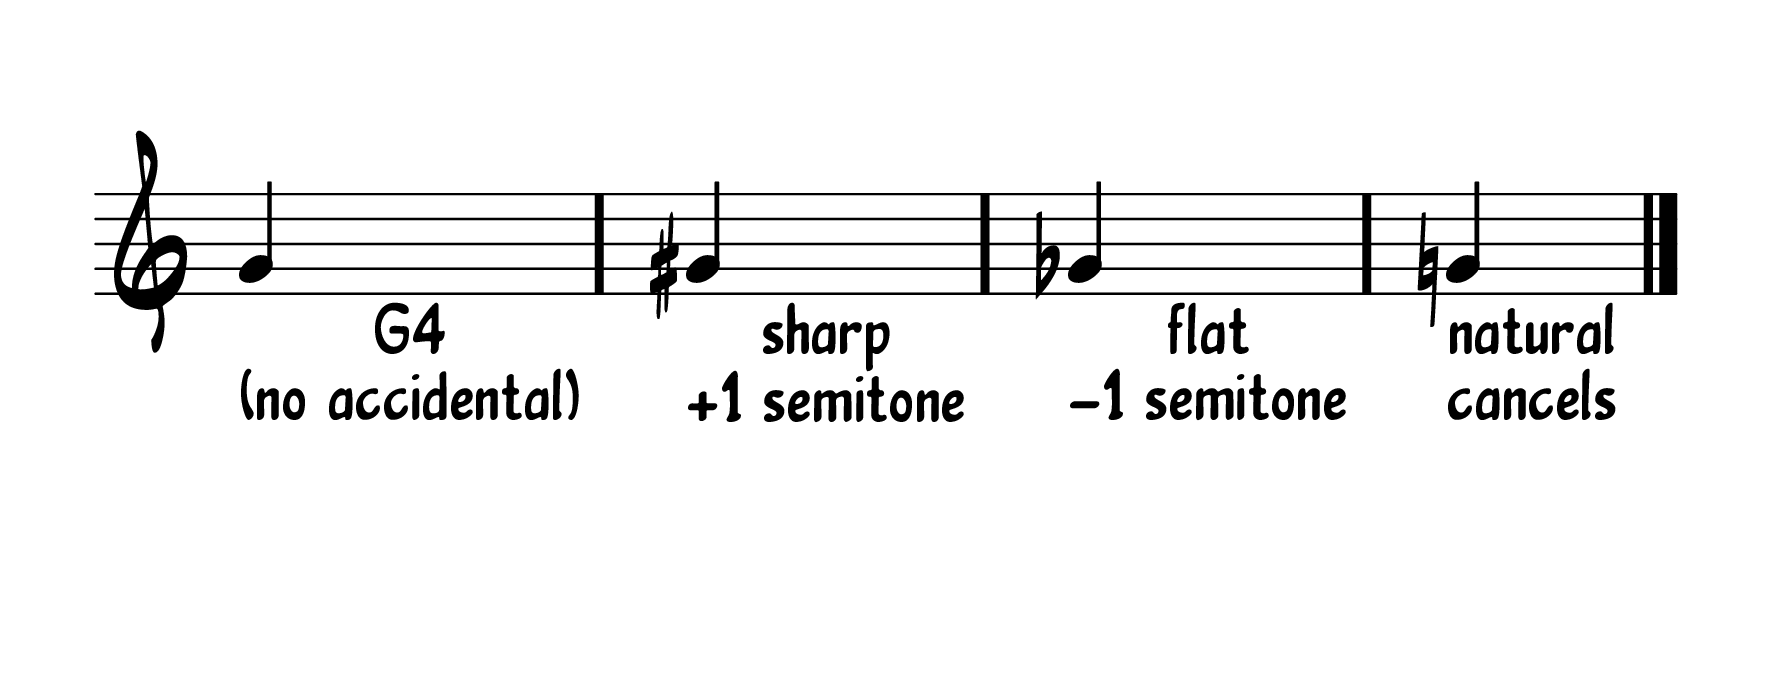
\includegraphics[width=0.82\textwidth]{figures/fig_accidentals}
    \caption{The three accidentals applied to G4, rendered in LilyJAZZ notation:
    a \term{sharp} raises the pitch one semitone, a \term{flat} lowers it one semitone,
    and a \term{natural} cancels a previous accidental.
    The leftmost note carries none.}
    \label{fig:accidentals}
\end{figure}

A \term{key signature}, printed once just after the clef, applies a fixed set of sharps or
flats to every occurrence of the affected letters throughout the piece, sparing the writer
from marking each note individually.
Two sharps, for instance, denotes D major: every F and C is played as F\(\sharp\) and
C\(\sharp\) unless a natural overrides it locally.
Signatures range from seven flats to seven sharps, with C major in the middle carrying
none.
\Cref{fig:key-signatures} shows four common signatures on the treble staff.

\begin{figure}[htbp]
    \centering
    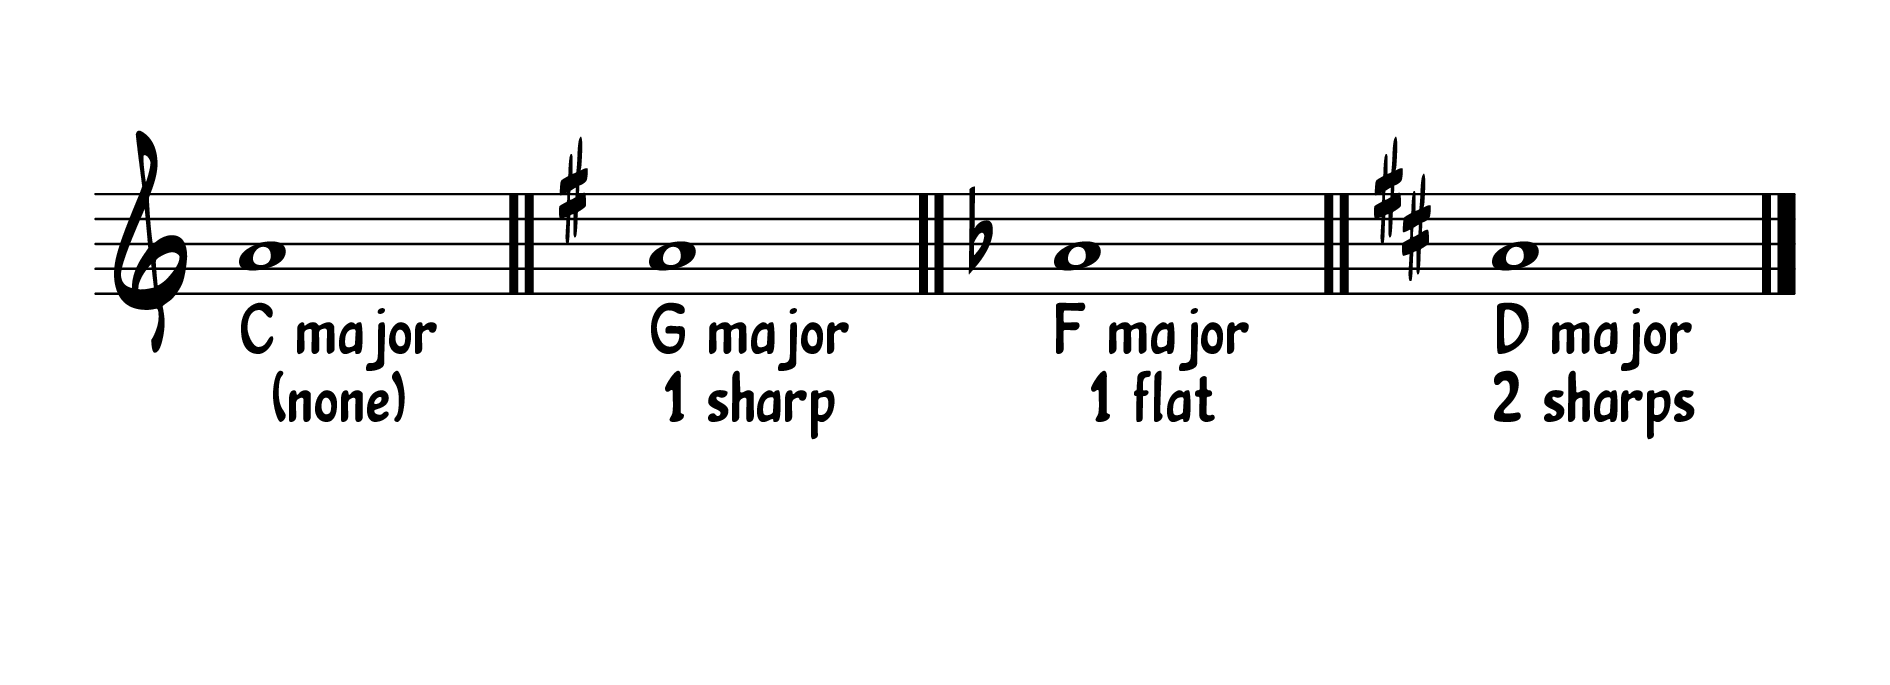
\includegraphics[width=0.88\textwidth]{figures/fig_key_signatures}
    \caption{Four key signatures on the treble staff, rendered in LilyJAZZ notation:
    C major (no accidentals), G major (one sharp), F major (one flat), and D major
    (two sharps).
    The anchor note is the same in every measure; only the signature at the clef
    changes.}
    \label{fig:key-signatures}
\end{figure}

\section{Note and Rest Durations}

A note's duration is read from three cues on its body, summarised in
\Cref{tab:note-durations}.
The \emph{notehead} is open (hollow) for the two longest values and filled (solid) for
quarter notes and shorter.
The \emph{stem and flags} refine this: a whole note has no stem, every other note has one,
and each \term{flag} added to the stem halves the value (one flag is an eighth, two a
sixteenth, three a thirty-second).
Consecutive flagged notes usually have their flags merged into a horizontal \term{beam},
which groups them visually without changing any duration.
Finally, an \term{augmentation dot} to the right of the notehead lengthens it by half its
own value, so a dotted quarter equals a quarter plus an eighth.

\begin{table}[htbp]
    \centering
    \caption{Standard note values and how each is drawn.
    The duration is read from the notehead, the stem and its flags, and any augmentation
    dot; the final column gives the value in beats when the quarter note is the beat, as
    in 4/4.}
    \label{tab:note-durations}
    \small
    \setlength{\tabcolsep}{8pt}
    \renewcommand{\arraystretch}{1.2}
    \begin{tabular}{@{} l l l c c @{}}
        \toprule
        \textbf{Value} & \textbf{Notehead} & \textbf{Stem and flags} &
        \textbf{Whole-note fraction} & \textbf{Beats in 4/4} \\
        \midrule
        Whole         & open   & none              & \(1\)    & \(4\)   \\
        Half          & open   & stem              & \(1/2\)  & \(2\)   \\
        Quarter       & filled & stem              & \(1/4\)  & \(1\)   \\
        Eighth        & filled & stem, 1 flag      & \(1/8\)  & \(1/2\) \\
        Sixteenth     & filled & stem, 2 flags     & \(1/16\) & \(1/4\) \\
        Thirty-second & filled & stem, 3 flags     & \(1/32\) & \(1/8\) \\
        \addlinespace
        Dotted quarter & filled & stem, dot           & \(3/8\)  & \(3/2\) \\
        Dotted eighth  & filled & stem, 1 flag, dot   & \(3/16\) & \(3/4\) \\
        \bottomrule
    \end{tabular}
\end{table}

\term{Rests} mark silence and follow the same value hierarchy as notes, each with its own
glyph; a \term{whole-measure rest}, a filled block hanging under a staff line, empties
an entire measure regardless of the time signature.
\Cref{fig:note-durations} shows the note values side by side.

\begin{figure}[H]
    \centering
    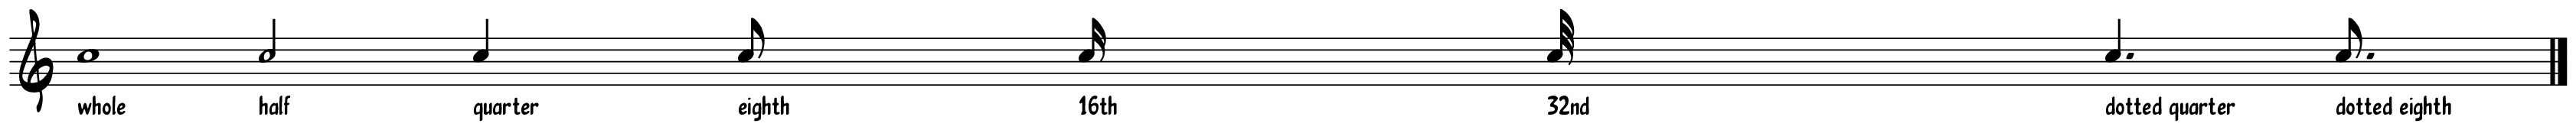
\includegraphics[width=1\textwidth,height=\TFGmusicStaffDispHeight,keepaspectratio]{figures/fig_note_durations}
    \caption{Note duration values rendered in LilyJAZZ notation, from left to right:
    whole, half, quarter, eighth, sixteenth, thirty-second, dotted quarter, and dotted
    eighth.
    The open notehead with no stem encodes the longest value (whole note); each
    flag added to the stem halves the duration; an augmentation dot extends it by
    half.}
    \label{fig:note-durations}
\end{figure}

\section{Time Signatures and Measures}

Vertical \term{barlines} divide the staff into \term{measures} (or \term{bars}), each
holding the same total duration.
That total is set by the \term{time signature}, a pair of stacked numbers at the start of
the piece (repeated only when it changes): the upper number counts the beats per measure,
and the lower number names the note value of one beat (4 for a quarter, 8 for an eighth,
2 for a half).
So 4/4 is four quarter-note beats per bar, while 6/8 is six eighth notes felt as two
groups of three.

The jazz repertoire is overwhelmingly written in 4/4, but the Real Book also uses the
seven other signatures in \Cref{tab:time-sigs}; together these eight constitute the
in-scope set of this thesis (\Cref{sec:scope}).

\begin{table}[htbp]
    \centering
    \caption{The eight time signatures that occur in the in-scope repertoire.
    The upper number counts the beats per measure and the lower number names the beat
    unit.}
    \label{tab:time-sigs}
    \small
    \setlength{\tabcolsep}{8pt}
    \renewcommand{\arraystretch}{1.2}
    \begin{tabular}{@{} l l l @{}}
        \toprule
        \textbf{Signature} & \textbf{Contents of one measure} & \textbf{Common name / use} \\
        \midrule
        4/4  & four quarter notes                          & common time (most of the repertoire) \\
        3/4  & three quarter notes                         & waltz \\
        2/4  & two quarter notes                           & march, fast two-feel \\
        2/2  & two half notes                              & cut time \\
        6/8  & six eighth notes (two groups of three)      & compound duple \\
        6/4  & six quarter notes (two groups of three)     & compound duple (slow) \\
        5/4  & five quarter notes                          & odd metre \\
        12/8 & twelve eighth notes (four groups of three)  & compound quadruple (ballads) \\
        \bottomrule
    \end{tabular}
\end{table}

\section{Chord Symbols}
\label{sec:chord-symbols-primer}

Above the melody, jazz scores print \term{chord symbols} roughly aligned to the beat where
each harmony begins; they tell the rhythm section and the improvising soloist what to play
under the tune.
A chord symbol is compact free-form text with up to four parts, listed in
\Cref{tab:chord-anatomy}: an obligatory \emph{root}, an optional \emph{quality}, optional
\emph{extensions or alterations}, and an optional \emph{slash bass}.
The parts combine left to right.
Reading \texttt{F\#m7b5}, for example: root F\(\sharp\), quality \texttt{m7} (minor
seventh), alteration \texttt{b5}, together the half-diminished chord; and \texttt{C/E}
is a C major triad voiced over an E in the bass.

\begin{table}[htbp]
    \centering
    \caption{The four parts of a jazz chord symbol.
    Only the root is obligatory; the remaining parts are optional and are concatenated left
    to right.}
    \label{tab:chord-anatomy}
    \small
    \setlength{\tabcolsep}{8pt}
    \renewcommand{\arraystretch}{1.2}
    \begin{tabular}{@{} l l l @{}}
        \toprule
        \textbf{Part} & \textbf{Meaning} & \textbf{Examples} \\
        \midrule
        Root                     & pitch class A--G, optional accidental & \texttt{C}, \texttt{F\#}, \texttt{Bb} \\
        Quality                  & chord-type abbreviation               & \texttt{maj7}, \texttt{m7}, \texttt{7}, \texttt{m7b5}, \texttt{dim7} \\
        Extensions / alterations & added or altered chord tones          & \texttt{\#9}, \texttt{b5}, \texttt{13} \\
        Slash bass               & non-root note placed in the bass      & \texttt{/E} in \texttt{C/E} \\
        \bottomrule
    \end{tabular}
\end{table}

Because chord symbols are text rather than staff glyphs, recovering them is an
\term{optical character recognition} (OCR) problem distinct from the staff-pattern
recognition used for the melody. This split motivates the two-stream architecture of
\Cref{ch:design}.

\section{The Lead-Sheet Format}

A jazz lead sheet assembles the elements above into a minimal score: one or more
\term{systems} of single-voice treble-clef staff carrying the melody (each opening with
a clef, key signature, and time signature), chord symbols above the staff, and
sometimes structural marks such as repeat signs, section labels (\textit{A},
\textit{B}, \textit{Bridge}), or style indications.
Many of these marks are absent from informal editions, including large parts of
\textit{The Real Book}.
\Cref{fig:leadsheet-example} shows a clean synthetic rendering in the LilyJAZZ style used
to train the system, and \Cref{fig:realbook-annotated} an actual Real Book page with its
elements labelled.

\begin{figure}[htbp]
    \centering
    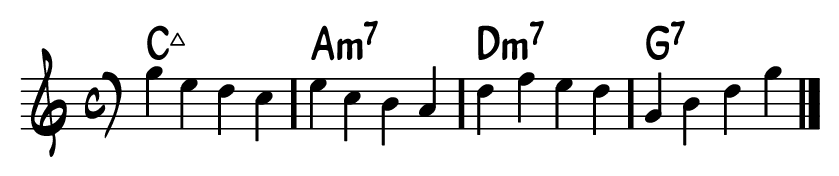
\includegraphics[width=1\textwidth]{figures/fig_leadsheet_excerpt}
    \caption{A four-bar jazz lead-sheet excerpt in C major (4/4), rendered in
    LilyJAZZ style, the same engraving used to generate the synthetic training
    dataset.
    Chord symbols above the staff (\texttt{Cmaj7}, \texttt{Am7}, \texttt{Dm7},
    \texttt{G7}) encode the I--vi--ii--V harmonic progression; the melody line
    encodes pitch through vertical position and duration through notehead shape
    and stem.}
    \label{fig:leadsheet-example}
\end{figure}

\begin{figure}[htbp]
    \centering
    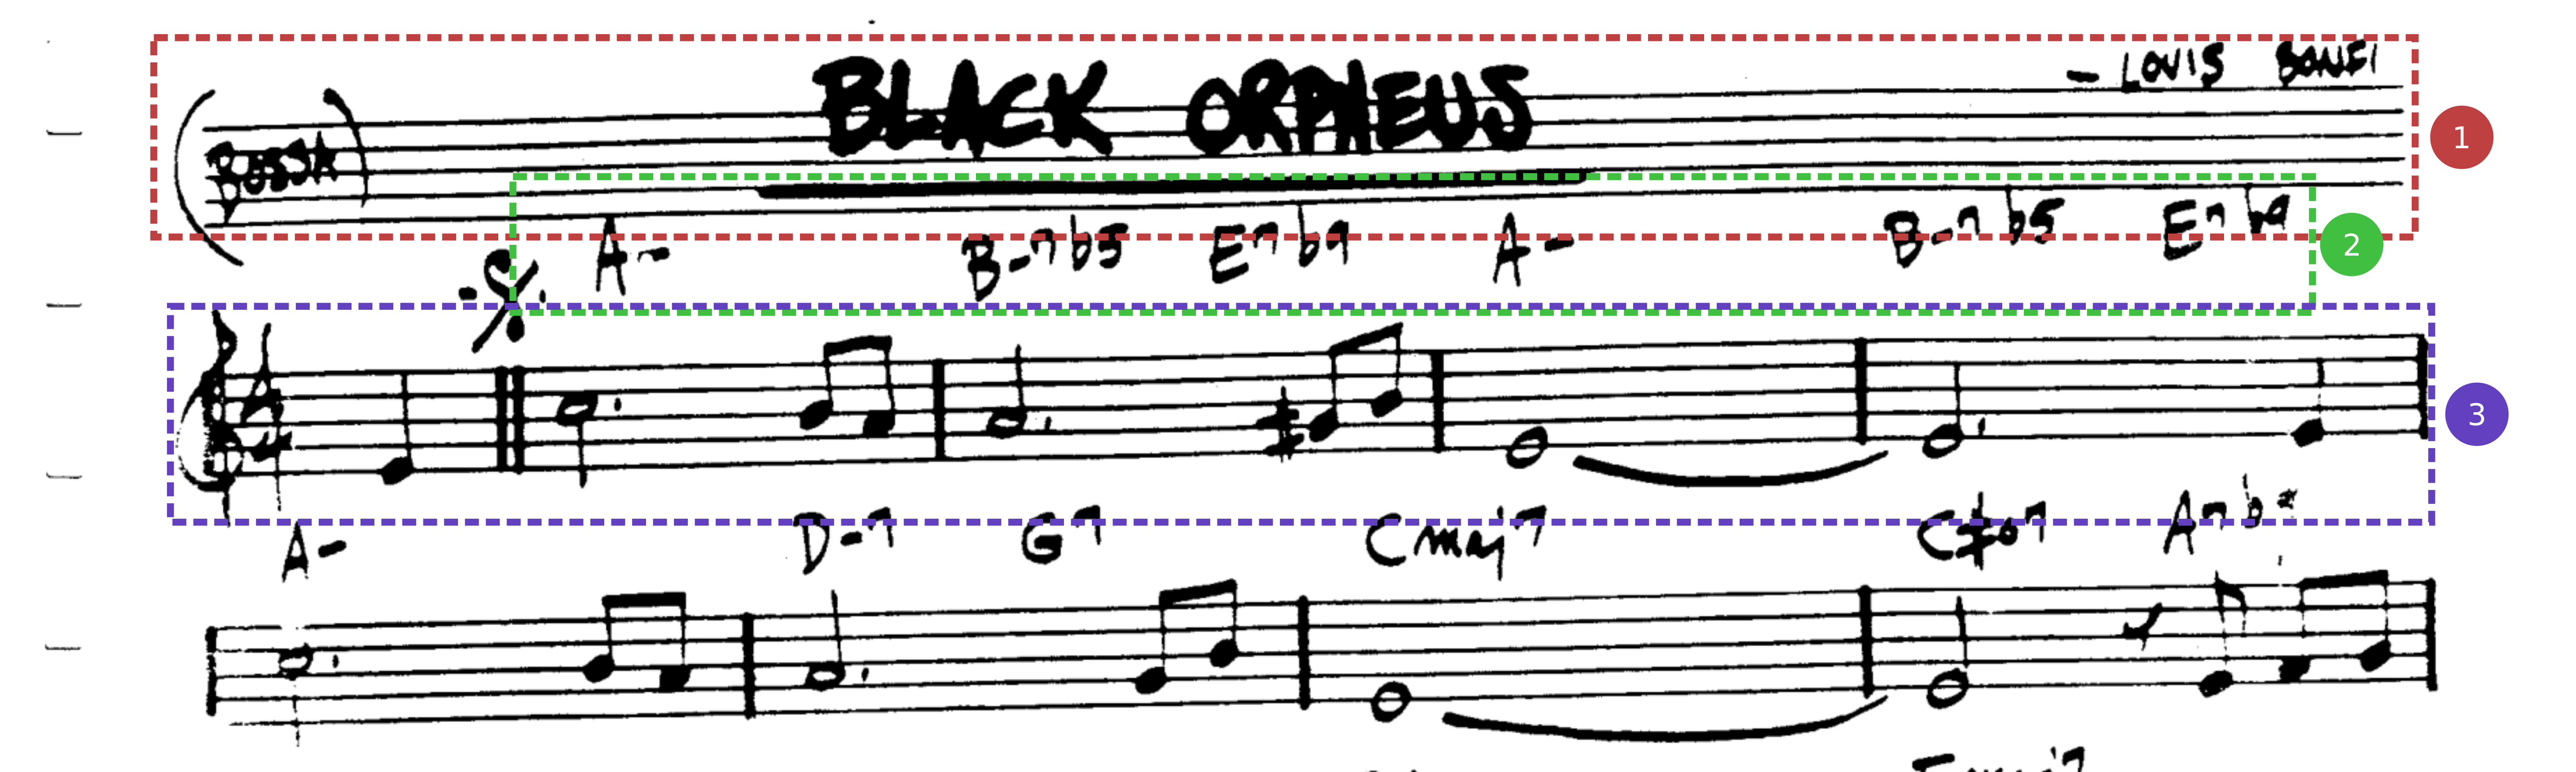
\includegraphics[width=\textwidth]{figures/fig_realbook_labeled}
    \caption{Excerpt from \textit{The Real Book} (``Black Orpheus'', L.\ Bonfá),
    showing the hand-engraved notation the OMR system must transcribe: \textbf{(1)} Header metadata. \textbf{(2)} Chord symbol regions targeted by the OCR stream. \textbf{(3)} Monophonic staff systems targeted by the CRNN-CTC model.}
    \label{fig:realbook-annotated}
\end{figure}
